\section{Úvod}

Podstatou projektu v~předmětu BPC-PRP je využít již sestaveného robota a implementovat postupně řešení tří úkolů (jízdy po čáře, jízdy uprostřed koridoru a úniku z~bludiště).

% popis robota
Připravený robot (viz Obrázek \ref{fig:robot_obr}) se pohybuje s~využitím diferenciálního podvozku, kde obě kola pohání motory propojené pro zajištění zpětné vazby s~rotačními enkodéry. Pro sledování čáry je vybaven dvěma infračervenými senzory, pro jízdu v~koridoru a vyhýbání se překážkám pak může využít rotační LiDAR a tři ultrazvukové senzory vzdálenosti. Dále může využít IMU, kameru, tři integrovaná tlačítka a čtyři RGB LED (především pro signalizaci svého stavu), viz také návod k~sestavení robota \cite{robot}.

% spojení s PC
Na robotovi se nachází počítač Raspberry Pi, na kterém běží systém ROS2 \cite{ros}. S~tímto počítačem komunikuje přes WiFi uživatelský počítač, kde je (opět s~pomocí ROS2) spouštěn program ovládající činnost robota. 

\begin{figure}[h]
    \centering
    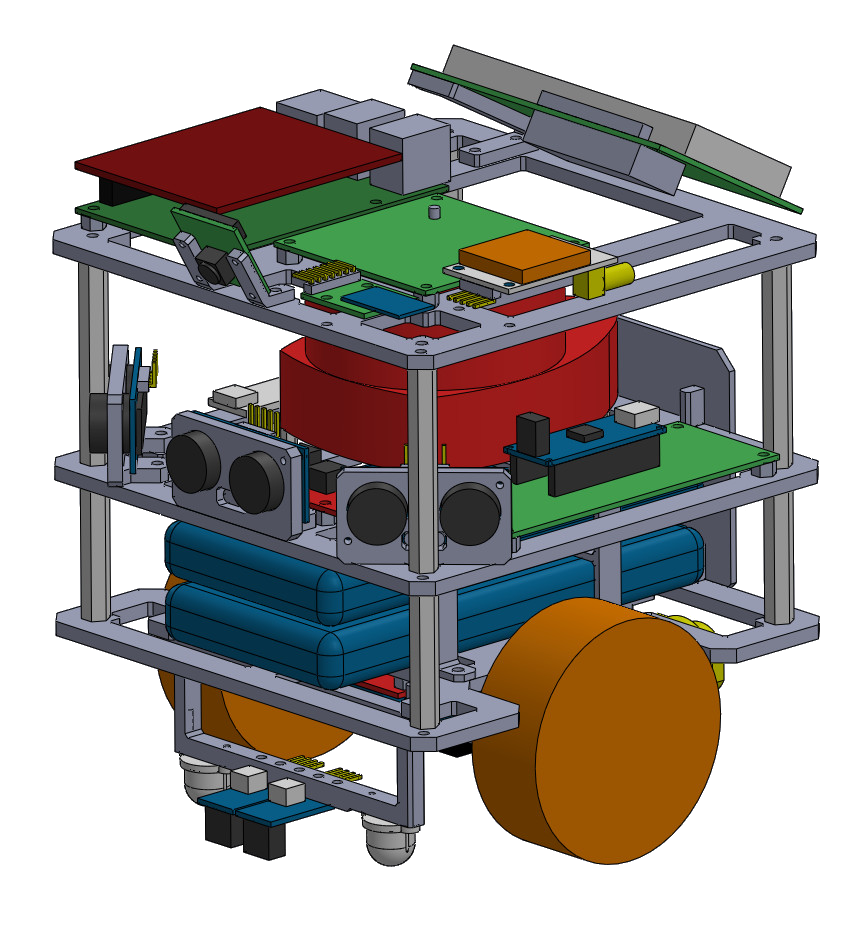
\includegraphics[width=0.35\textwidth]{images/fenrir.png}
    \caption{Model robota (převzato z~\cite{prez1})}
    \label{fig:robot_obr}
\end{figure}

% popis úkolů
Prvním úkolem robota je za pomoci infračervených senzorů sledovat čáru (tj. jet podél ní). Čára je v~jednom případě rovná, v~druhém případě tvoří kruh a v~posledním případě tvoří obrys čísla 8. Druhým úkolem je, s~využitím LiDARu, ultrazvukových senzorů nebo kombinace obojího, projet koridorem tak, aby se robot držel uvnitř a nedotýkal se stěn. Chodby mají stejné tvary jako čáry, tedy linie, kruh a osmička. Posledním úkolem je (zjednodušeně) s~využitím libovolných senzorů robota a libovolné strategie projet bludištěm. Bludiště je tvořeno již známými koridory, kde se před každou křižovatkou vedoucí k~cíli nachází ArUco kód napovídající správný směr odbočení. Kompletní pravidla jsou k~dispozici v~kapitolách 2.8, 2.12 a 2.13 zadání laboratoří a zkoušek \cite{lab}.
